El análisis de componentes principales no produce resultados de calidad si la relación entre las variables aleatorias es no lineal.
Los algoritmos de \textit{manifold learning} convierten los conjuntos de datos en otros de menor dimensionalidad conocidos como \textbf{manifolds}, obtenidos aplicando transformaciones no lineales sobre el espacio original de estos.

A continuación se mencionan algunos de los algoritmos de manifold learning más conocidos.

\subsection{Multi-dimensional Scaling}\label{subsec:MDS}

\textit{Multi-dimensional scaling} (MDS) es una técnica que tiene como objetivo obtener una representación del conjunto de datos en un espacio de menos dimensiones, preservando las distancias existentes entre los elementos en el espacio original.

En otras palabras, se busca minimizar la siguiente función objetivo:

\begin{equation}
    \label{eq:MDS}
    \sum_{i=1}^{N}\sum_{j=i+1}^{N}{d_{ij} - \hat{d}_{ij}}
\end{equation}

\noindent
dado un conjunto de datos de $N$ elementos, donde $d_{ij}$ y $\hat{d}_{ij}$ son las distancias entre los elementos $i$ y $j$ en los espacios original y reducido respectivamente.

Puesto que MDS se basa en las distancias entre los elementos y no utiliza la representación vectorial de estos, esta técnica puede emplearse incluso en casos en los que el conjunto de datos no posee tal representación (por ejemplo, cadenas de texto), siempre que la distancia o similitud entre ellos haya sido definida.

\subsection{Isomap}\label{subsec:isomap}

Al igual que PCA, MDS tampoco produce buenos resultados cuando la relación entre los puntos no es lineal.
\textit{Isomap} puede considerarse como una extensión de MDS, desarrollada para procesar ese tipo de conjuntos de datos; y que a diferencia de MDS, se basa en la distancia \textit{geodésica} entre los puntos.

Para ello se construye un grafo donde existirá una arista entre los puntos $i$ y $j$ si estos son \textit{vecinos} en el espacio original, que tendrá un peso igual a la distancia euclidiana entre los puntos.

Luego la distancia geodésica entre cualquier par de puntos se corresponderá con el camino de costo mínimo entre estos en el grafo.
Finalmente, empleando esta nueva distancia, se aplica MDS\@.

El modo en que se determina si dos puntos son vecinos entre sí, está sujeto a variaciones.
Generalmente suele definirse un cierto radio para el que si dos puntos se encuentran a una distancia menor que este, se consideran vecinos.
Otro enfoque consiste en, dado un valor $k$, fijar como vecinos de un punto los $k$ puntos más próximos a este.

\begin{figure}[!h]
    \centering
    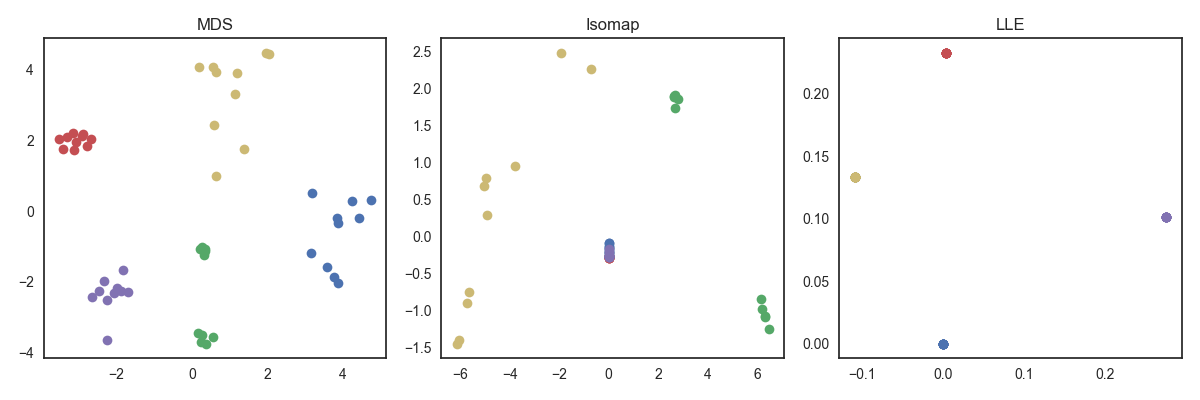
\includegraphics[width=\textwidth]{manifold-learning.png}
    \caption{Resultado de aplicar diferentes algoritmos de \textit{manifold learning} para reducir a dos las dimensiones del mismo conjunto de datos usado en la figura~\ref{img:pca}.}
    \label{img:manifold-learning}
\end{figure}

\subsection{Locally Linear Embedding}\label{subsec:LLE}

\textit{Locally Linear Embedding} (LLE) es una técnica para la reducción de dimensiones basada en la idea de analizar regiones locales de puntos superpuestas, para determinar la estructura local de los datos.

El primer paso del algoritmo consiste en hallar los puntos más cercanos a cada punto $x_i$, expresando luego a $x_i$ como una combinación lineal de estos.
De modo que se cumpla que $x_i =\sum_j {w_{ij}x_j}$, donde $\sum_j w_{ij}=1$ y $w_{ij} = 0$ si $x_j$ no es un vecino cercano de $x_i$.
La matriz de pesos $W$, de coeficientes $w_{ij}$ es encontrada minimizando el error cuadrático medio, dado por la ecuación:

\begin{equation}
    error(W) = \sum_i \left( x_i - \sum_j {w_{ij}x_j} \right)^2
\end{equation}

Luego, la reducción de dimensiones se realiza a partir de la matriz $W$ y un número de dimensiones $p$ prefijado.
Para ello, si $y_i$ es el vector correspondiente a $x_i$ en el nuevo espacio, y $Y$ matriz que tiene a los vectores $y_i$ como filas;
entonces se busca $Y$ tal que minimice la siguiente expresión:

\begin{equation}
    error(Y) = \sum_i \left( y_i - \sum_j {w_{ij}y_j} \right)^2
\end{equation}

Es decir, la nueva representación del conjunto de datos minimiza el error cuadrático medio a partir de los pesos encontrados para la representación original.

% TODO Consider to remove this
%\subsection{t-distributed Stochastic Neighbor Embedding}\label{subsec:TSNE}
%
%\textit{t-distributed Stochastic Neighbor Embedding} (t-SNE)~\cite{vanderMaaten08} es un algoritmo de manifold learning especialmente diseñado para la visualización en dos o tres dimensiones de conjuntos de datos multidimensionales.
%t-SNE representa las similitudes de los datos en su espacio original como probabilidades condicionales, que siguen una distribución Gaussiana;
%y modela la similitud entre los datos en el espacio transformado (de menor dimensión) utilizando probabilidades condicionales que siguen una distribución t-Student.
%
%Para determinar la representación del conjunto de datos en el nuevo espacio, el algoritmo minimiza la \textit{divergencia de Kullback-Leibler}~\cite{vanderMaaten08} entre las probabilidades